\chapter{Estado de Arte}
\label{chap:estado-de-arte}
En este capítulo analizaremos diferentes investigaciones sobre question answering para poder ilustrarnos acerca de los distintos problemas y las distintas formas de encararlos que existen. Discutiremos primero una serie de investigaciones académicas pequeñas, presentadas en general en congresos y competencias del área para inferir un modelo más o menos general del dominio de problemas y los acercamientos típicos. Luego, comentaremos el sistema de IBM -Watson- para ilustrarnos, más allá de los enfoques usuales, un enfoque exitoso. Finalmente pasaremos revista de una serie de sistemas disponibles para facilitar la creación de modelos de question answering, haciendo foco en Qanus (un framework que de hecho pudimos utilizar durante un periodo de nuestra investigación) y mencionando algunos sistemas que evaluamos teóricamente pero que, lamentablemente, no estaban disponibles \textit{out of the box}, principalmente debido a restricciones y modificaciones en el acceso programático que implementaron los buscadores populares en los últimos años\footnote{Ver por ejemplo, Google Search API, deprecado el 1ero de noviembre de 2010 aquí: https://developers.google.com/web-search/}

\section{IBM-Watson}

Watson es un sistema diseñado por IBM con el objetivo de competir en
tiempo real en el programa de televisión estadounidense Jeopardy,
logrando resultados del nivel de los campeones humanos de este
programa.

El proyecto demoró 3 años de investigación, en los cuales se
logró obtener la performance esperada (nivel humano experto) en
cuanto a precisión, confiabilidad y velocidad, logrando derrotar a
dos de los hombre con mayores récords históricos del show en un
programa en vivo [MáS DATOS -LINKS]

El objetivo del \ proyecto puede considerarse una extensión de lo que
fue Deep Blue, el sistema que logró el nivel de los expertos humanos
en el ajedrez, porque buscó superar un reto que significativo y
visible del campo de la Inteligencia Artificial tanto para la comunidad
científica como para la sociedad en general:
{\textquotedblleft}?`puede un sistema computacional ser diseñado para
competir con los mejores hombre en alguna tarea que requiera altos
niveles de inteligencia humana y, si es el caso, que clase de
tecnología, algoritmos e ingenieria se
requiere?{\textquotedblright}\footnote{\ Traducción propia de
Building Watson: An Overview of the DeepQA Project, p2}

Watson es la implementación específica para participar en este
programa de una arquitectura más genérica de question answering,
DeepQA, que da el nombre al proyecto de la corporación. Esta
arquitectura ejemplifica perfectamente la complejidad del problema de
QA de dominio abierto e incorpora tecnologías de punta de distintos
dominios de ciencias de la computación, y de IA en particular:
information retrieval, natural language processing, knowledge
representation and reasoning, machine learning e interfaces humano -
computadora.

\subsection{El problema}

Watson debe realizar tareas como parsing, question classification,
question descomposition, automatic source adquisition and evaluation,
entity and relation detection, logical form generation, knowledge
representation and reasoning manteniendo ciertos atributos de calidad
bastante exigentes derivados de la naturaleza del show. Estas
restricciones son:

\begin{itemize}
\item Confiabilidad de la respuesta: \newline
Jeopardy tiene tres participantes con un pulsador y el que desee
responder debe pulsar antes que los demás. Además, existe una
penalización por respuestas incorrectas, por lo que es esencial que
el sistema pueda determinar la confiabilidad de la respuesta obtenida a
fin de optar por responder o no responder.
\item Tiempos de respuesta: \newline
La confiabilidad de la respuesta, o al menos una estimación, debe
calcularse antes de que pase el tiempo para decidir responder (6
segundos) y también de que otro participante oprima su pulsador
(menos de 3 segundos).
\item Precisión:\newline
El tipo de respuestas que se dan en el show suelen ser respuestas
exactas (por ejemplo: solamente un nombre, un número o una fecha,
etc). 
\end{itemize}

\bigskip

El sistema cuenta con varios componentes heurísticos que estiman
ciertos features y grados de confiabilidad para diferentes respuestas,
los cuales son evaluados por un sistema general que sintetiza un grado
de confiabilidad para una respuesta final y determina así si
responder o no responder. 

El programa consta de un tablero con 30 pistas (o preguntas) organizadas
en seis columnas, cada una de las cuales es una categoría. Las
categorías van desde temas acotados como
{\textquotedblleft}historia{\textquotedblright} o
{\textquotedblleft}ciencias{\textquotedblright} hasta temas más
amplios como {\textquotedblleft}cualquier cosa{\textquotedblright} o
{\textquotedblleft}potpourri{\textquotedblright}. Watson intenta
respuestas sobre varias hipótesis de dominio y verifica en cual de
ellos se logran respuestas de mayor confiabilidad. 

Por otra parte, el grueso de las preguntas de Jeopardy son del tipo
\textit{factoid}, esto es, preguntas cuya respuesta esta basada en
información fáctica acerca de una o más entidades individuales.


\bigskip

Por ejemplo:

Categoría: Ciencia General

Pista: Cuando es impactado por electrones, un fósforo emite energía
electromagnética de esta forma

Respuesta: Luz (o fotones)


\bigskip

A su vez, existen ciertos tipos de pistas que requieren un enfoque
particular, por ejemplo, pistos que constan de dos subpistas muy
débilmente relacionadas, o problemas matemáticos formulados en
lenguaje humano, o problemas de fonética, etc, que no pueden ser
simplemente dejados de lado porque, si bien tiene poca probabilidad de
aparición, cuando aparecen lo hacen en bloque y pueden arruinar el
juego de Watson. Se acordó con la productora del programa, sin
embargo, dejar de lado preguntas audiovisuales (aquellas que presentan
una imagen o un audio y requieren interpretarlo) y preguntas que
requieren instrucciones verbales del presentador.


\bigskip

Para determinar el dominio de conocimiento, los investigadores
analizaron 20000 preguntas, extrayendo su LAT (lexical answer type, o
tipo léxico de respuesta). El LAT se define como una palabra en la
pista que indica el tipo de la respuesta esperado. Por ejemplo, para la
pista {\textquotedblleft}Investanda en 1500{\textquoteright}s para
agilizar el juego, este movimiento involucra dos
piezas{\textquotedblright} el LAT es
{\textquotedblleft}movimiento{\textquotedblright}. Menos del 12\% de
las pistas no indicaba explícitamente ningún LAT, usando palabras
como {\textquotedblleft}esto{\textquotedblright} o
{\textquotedblleft}eso{\textquotedblright}. En estos casos, el sistema
debe inferir el tipo de respuesta del contexto. Del análisis de estas
20000 pistas se reconocieron 2500 tipos léxicos distintos, de los
cuales los 200 más frecuentes no llegaban a cubrir el 50\% del total
de pistas. Esto implica que un approach estructurado (orientado por el
tipo de respuesta), si bien resulta útil para algunos tipos, no es
suficiente para abordar el problema completo.

\subsection{Métricas}

Las métricas de resultados, además del tiempo de respuesta, son la
\textit{precisión} (preguntas contestadas correctamente / preguntas
contestadas) y el \textit{porcentaje de respuestas dadas }(preguntas
contestadas / total de preguntas). Mediante la configuración de un
threshold de \textit{confiabilidad} pueden obtenerse distintas
estrategias de juego: un umbral bajo repercutirá en un juego más
agresivo, incrementando la proporción de respuestas contestadas,,
pero disminuyendo su precisión, mientras que un umbral alto
determinará un juego conservador, con menos respuestas dadas pero
mayor precisión en las mismas. Es un clásico escenario de trade-off
entre dos atributos de calidad. Un buen sistema de estimación de
confiabilidad implica una mejora general del sistema, aún cuando el
módulo de generación de respuestas permanezca idéntico.


\bigskip

En el show, el porcentaje de respuestas dadas depende de la velocidad
con la que se llega a presionar el pulsador, lo cual sólo interesa
para el dominio de QA como una restricción temporal. 


\bigskip

Mediante análisis numérico, los investigadores determinaron que los
campeones de Jeopardy lograban tomar entre el 40\% y el 50\% de las
preguntas y, sobre ellas, lograban una precisión de entre el 85\% y
el 95\%, lo que determinaba una barrera de performance bastante
exigente en lo que respecta a QA.


\bigskip

\subsection{Baseline}

El equipo de IBM intentó utilizar dos sistemas consolidados en QA y
adaptarlos al problema \ de Jeopardy. \ El primero fue PIQUANT
(Practical Intelligent Question Answering Technology), un sistema
desarrollado por IBM en conjunto con el programa del gobierno
estadounidense AQUAINT y varias universidades, que estaba entre los
mejores según la TREC (Text Retrieval Conference), una autoridad en
el área. PIQUANT consta de un pipeline típico (véase QANUS) con
tecnología de punta, logrando un rango del 33\% de respuestas
correctas en las evaluaciones TREC-QA. Los requerimientos de la
evaluación de TREC son muy distintos de los de Jeopardy: TREC ofrece
un corpus de conocimiento relativamente pequeño (1M de documentos) de
donde las respuestas deben ser extraídas y justificadas, el tipo de
preguntas de TREC son menos complejas a nivel ling\"uístico que las
de Jeopardy y la estimación de confiabilidad no resulta una métrica
importante (dado que no hay penalización por respuestas incorrectas).
Además, los sistemas tienen permitido acceder a la web y las
restricciones temporales son, por mucho, más amplias (por ejemplo:
una semana para responder 500 preguntas). En Jeopardy, además de las
restricciones ya mencionadas, un requerimiento fue que el sistema
trabaje sobre datos locales y no acceda a la web en tiempo real. El
intento de adaptar PIQUANT al problema de Jeopardy dio pésimos en
comparación con los necesarios: 47\% de precisión sobre el 5\% de
respuestas con mayor confiabilidad y 13\% de precisión en general. 

Por otro lado, el equipo intentó adaptar el sistema OpenEphyra
(véase OpenEphyra), un framework open-source de QA desarrollado en
CMU (Carnegie Mellon University) basado en Ephyra (no libre),
diseñado también para la evaluación TREC. OpenEphyra logra un
45\% de respuestas correctas sobre el set de datos de evaluación TREC
2002, usando busqueda web. La adaptación resultó aún peor que la
de PIQUANT (con menos del 15\% de respuestas correctas y una mala
estimación de la confiabilidad). 

Se probaron dos adaptaciones de estos sistemas. una basada en
búsquedas de texto puro y otra basada en reconocimiento de entidades.
En la primera, la base de conocimiento se modeló de manera no
estructurada y las preguntas se interpretaron como términos de una
query, mientras que en la segunda se modeló una base de conocimientos
estructurada y las preguntas se analizaron semánticamente para
reconocer entidades y relaciones, para luego buscarlos en la base.
Comparando ambos enfoques en base al porcentaje de respuestas dadas, el
primero dio mejores resultados para el 100\% de las respuestas,
mientras que la confiabilidad general era baja; por otro lado, el
segundo enfoque logró altos valores de confiabilidad, pero sólo en
los casos en que efectivamente logra identificar entidades. De aquí
se infiere que cada enfoque tiene sus ventajas, en el dominio de
problemas apropiado.

\subsection{La arquitectura DeepQA}
\label{subsec:deep-qa}
Los intentos de adaptación iniciales, como vimos, no dieron
resultados, así como tampoco sirvieron las adaptaciones de algoritmos
de la literatura científica, los cuales son realmente difíciles de
sacar de su contexto original y de las evaluaciones sobre las cuales
fueron testeados. Este problema, veremos -por ejemplo, con QANUS y
Reverb- , se repitió en nuestro proyecto. Como conclusión de estos
intentos frustrados, el equipo de IBM entendió que una arquitectura
de QA no debía basarse en sus componentes concretos sino en la
facilidad para incorporar nuevos componentes y para adaptarse a nuevos
contextos. Así surgió DeepQA, la arquitectura de base, de la cual
Watson es una instancia concreta para un contexto particular (con
requerimientos de alta precisión, buena estimación de
confiabilidad, lenguaje complejo, amplitud de dominio y restricciones
de velocidad). DeepQA es una arquitectura de computo paralelo,
probabilistico, basado en recopilación de evidencia y scoring. Para
Jeopardy se utilizaron más de 100 técnicas diferentes para analizar
lenguaje natural, identificar y adjudicar valor a fuentes de
información, encontrar y generar hipótesis, encontrar y rankear
evidencias y mergear y rankear hipótesis en función de esta
evidencia. La arquitectura sirvió para ganar Jeopardy, pero también
se adaptó a otros contextos como la evaluación TREC, dando
resultados mucho mejores que sus predecesores. Los principios de
diseño subyacentes de la arquitectura son:

\begin{itemize}
\item Paralelismo masivo\newline
Para evaluar distintas hipótesis en distintos dominios con poco
acoplamiento.
\item Pervasive confidence estimation:\newline
Ningún componente genera la respuesta final, sino que da una serie de
features y grados de confiabilidad y evidencia para distintas
hipótesis, que luego son sintetizados.
\item Integrate shallow and deep knowledge:
\end{itemize}

\bigskip

A continuación, enumeraremos la lista de pasos que sigue el sistema
para obtener la respuesta a una pregunta:

\subsubsection{Adquisición de contenidos}

El primer paso de DeepQA es la adquisición de contenidos. Este paso es
el único que no se realiza en tiempo de ejecución y consiste en
crear la base de conocimiento en la cual el proceso final buscará la
respuesta a la pregunta, combinando subprocesos manuales y
automáticos. 

En principio se caracteriza el tipo de preguntas a responder y el
dominio de aplicación. El análisis de tipos de preguntas es una
tarea manual, mientras que la determinación del dominio puede
encararse computacionalmente, por ejemplo, con la detección de LATs
que señalamos antes. Dado el amplio dominio de conocimientos que
requiere Jeopardy, Watson cuenta con una gran cantidad de
enciclopedias, diccionarios, tesauros, artículos académicos y de
literatura, etc. A partir de este corpus inicial, el sistema busca en
la web documentos relevantes y los relaciona con los documentos ya
presentes en el corpus. 

Además de este corpus de documentos no estructurados, DeepQA maneja
contenidos semi-estructurados \ y estructurados, incorporando bases de
datos, taxonomías y ontologías como dbPedia, Wordnet y las
ontologías de Yago. 

\subsubsection{Análisis de la pregunta}

El primer paso en run-time es el análisis de la pregunta. En este paso
el sistema intenta entender qué es lo que la pregunta está
preguntado y realizar los primeros análisis que determinan cómo
encarará el procesamiento el resto del sistema. Watson utiliza
shallow parses, deep parses, formas lógicas, pos-tags,
correferencias, detección de entidades nombradas y de relaciones,
question classification, además de ciertos análisis concretos del
domiento del problema.

En este proceso se clasifica el tipo de la pregunta (los tipos están
determinados por el show: puzzles, matemáticos, etc). También se
busca el tipo de respuesta esperada, dónde los tipos manejados son
por Watson son los LATs extraídos de las preguntas de ejemplo. El LAT
determina el {\textquotedblleft}tipo{\textquotedblright} de la
respuesta, que clase de entidad \textit{es} la respuesta (una fecha, un
hombre, una relación, etc). El equipo de IBM intentó adaptar
distintos algoritmos de clasificación preexistentes, pero después
de intentar entrenarlos para el dominio de tipos de Jeopardy, llegaron
a la conclusión de que su eficacia era dependiente del su sistema de
tipos default, y que la mejor forma de adaptación era mappear su
output a los tipos utilizados por Watson (un enfoque similar fue
utilizado en esta tesis con respecto al clasificador de Stanford). Otra
anotación importante es el
{\textquotedblleft}foco{\textquotedblright} de la pregunta, la parte de
la pregunta tal que si se la reemplaza por la respuesta, la pregunta se
convierte en una afirmación cerrada.

Por ejemplo, para {\textquotedblleft}El hombre que escribió Romeo y
Julieta{\textquotedblright}, el foco es {\textquotedblleft}El hombre
que{\textquotedblright}. Este fragmento suele contener información
importante sobre la respuesta y al reemplazarlo por una respuesta
candidata se obtiene una afirmación fáctica que puede servir para
evaluar distintos candidatos y recolectar evidencia. Por ejemplo,
reemplazando por distintos autores y verificando que la oración
resultante esté presente en el corpus.

Por otro lado, muchas preguntas involucran relaciones entre entidades y,
más puntualmente, tienen una forma sujeto-verbo-objeto. Por ejemplo,
tomando la pista anterior, podemos extraer la relación
\textit{escribir(x, Romeo y Julieta)}. La amplitud del dominio de
Jeopardy hace que la cantidad de entidad y de relaciones entre
entidades sea enorme, pero esto empeora aún más al considerar las
distintas formas de expresar la misma relación. Por eso, Watson
sólo logra encontrar directamente una respuesta mediante
reconocimiento de entidades y relaciones sobre el 2\% de las pistas. En
general, este tipo de enfoque es útil sobre dominios más acotados,
mientras que la detección de relaciones como approach general a un
problema de question answering de dominio amplio es un área de
investigación abierta. 

Una particularidad ya señalada de las preguntas de Jeopardy son las
pistas con subpistas no relacionadas. Para atacar este problema, Watson
genera distintas particiones y resuelve todas en paralelo, sintetizando
las respuesta de cada partición generada mediante algoritmos ad-hoc
de ponderación de confiabilidad y otras características.

\subsubsection{Generación de hipótesis}

El tercer paso (segundo en run-time) es la generación de hipótesis:
tomando como input el resultado del paso anterior se generan respuestas
candidatas a partir de la base de conocimiento offline. Cada respuesta
candidata reemplazada por el foco de la pregunta es considerada una
hipótesis, que el sistema luego verificará buscando evidencias y
adjudicando un cierto grado de confiabilidad.

En la búsqueda primaria de respuestas candidatas, se busca generar
tantos pasajes como sea posible. El resultado final obtenido revela que
el 85\% de las veces, la respuesta final se encuentra entre los
primeros 250 pasajes devueltos por la búsqueda primaria. La
implementación utiliza una serie variada de técnicas, que incluyen
diferentes motores de búsqueda de textos (como Indri y Lucene),
búsqueda de documentos y de pasajes, búsquedas en bases de
conocimiento estructuradas como SPARQL con triple store y la
generación de mutiples queries a partir de una sola pregunta. La
búsqueda estructurada de triple stores depende del reconocimiento de
entidades y relaciones del paso anterior.

Para un número pequeño de LATs, se definió una suerte de conjunto
de entidades fijas (por ejemplo: países, presidentes, etc). Si la
respuesta final no es retornada en este paso, entonces no hay
posibilidad de obtenerla en los siguiente. Por eso se prioriza el
recall sobre la precisión, con el supuesto de que el resto del
pipeline logrará filtrar la respuesta correcta correctamente. Watson
genera varios cientos de hipótesis candidatas en este paso.


\bigskip

\subsubsection*{(Soft filtering)}

Para optimizar recursos, se realiza un filtrado liviano de respuestas
antes de pasar a la recopilación de evidencia y al scoring de
hipótesis. Un filtrado liviano es, por ejemplo, comprobar similaridad
de la respuesta candidata con el LAT esperado de la respuesta. Aquellas
hipótesis que pasan el filtro pasan al siguiente proceso, que realiza
un análisis más exhaustivo.


\bigskip

\subsubsection{Recuperación de evidencias y scoring de pasajes}

Para recuperar evidencias se utilizan varios algoritmos. Uno
particularmente útil es buscar la hipótesis candidata junto con las
queries generadas por la pregunta original, lo que señala el uso de
la respuesta en el contexto de la pregunta. \ Las hipótesis con sus
evidencias pasan al siguiente paso, dónde se les adjudica un score. 

El proceso de scoring es donde se realiza la mayor parte del análisis
más fuerte a nivel computacional. DeepQA permite la incorporación
de distintos Scorers, que consideran diferentes dimensiones en las
cuales la hipótesis sirve como respuesta a la pregunta original. Esto
se llevó a cabo definiendo una interfaz común para los scorers.
Watson incorpora más de 50 componentes que producen valores y
diferentes features basados en las evidencias, para los distintos tipos
de datos disponibles (no estructurados, semi estructurados y
estructurados). Los scorers toman en cuenta cuestiones como el grado de
similaridad entre la estrurctura de la respuesta y de la pregunta,
relaciones geoespaciales y temporales, clasificación taxonómica,
roles léxicos y semánticos que se sabe que el candidato puede
cumplir, correlaciones entre terminos con la pregunta, popularidad (u
obscuridad) de la fuente del pasaje, aliases, etc.

POR EJEMPLO: COPIAR NIXON

Los distintos scores se combinan luego en un score único para cada
dimensión.

(Merge)

Recién después de este momento, Watson realiza un merge entre
hipótesis idénticas. Las hipótesis idénticas son diferentes
formulaciones ling\"uisticas de lo mismo, por ejemplo:
{\textquotedblleft}X nació en 1928{\textquotedblright} o
{\textquotedblleft}El año de nacimiento de X es
1928{\textquotedblright}. Finalmente, se procede a estimar un ranking
único y una confiabilidad única para las distintas hipótesis. En
este paso se utilizan técnicas de machine learning que requieren
entrenamiento, y modelos basados en scores. Se utilizan técnicas
jerárquicas como mixture of experts y stacked generalization y,
finalmente, un metalearner fue entrenado para ensamblar los distintos
resultados intermedios. 


\bigskip

\subsection{Tiempos y escala}

DeepQA utiliza Apache UIMA, un framework que implementa UIMA
(Unestructured Information Management Architecture): todos los
componentes de DeepQA son IUMA-annotators, módulos que producen
anotaciones y aserciones sobre un texto.

La implementación inicial de Watson corría sobre un sólo
procesador y demoraba aproximadamente 2 horas en contestar una sola
pregunta. La arquitectura paralela permite, sin embargo, que al
correrlo sobre 2500 núcleos -de la implementación final- los
tiempos de respuesta oscilen entre 3 y 5 segundos, que es lo esperado.

Finalmente, la implementación de Watson logró alcanzar el estándar
de resultados de los campeones de Jeopardy y, como ya dijimos,
compitió y ganó el programa en Febrero de 2011. Además, se
realizaron adaptaciones para trabajar sobre los problemas de TREC, en
los cuales se demostró una amplia mejoría en comparación con
PIQUANT y OpenEphyra


\bigskip

\subsection{Conclusiones sobre IBM-Watson}

System level approach.


\bigskip

\section{La arquitectura de Qanus}

QANUS (Question-Answering @ National University of Singapore) es un
sistema de question answering basado en information retrieval. El
proyecto se actualizó por última vez en noviembre de 2012 y
contiene las herramientas más actuales de nlp (el POS-tagger, el
NER-tagger y el Question Classifier de Stanford) y también de
information retrieval índice de búsquedas lucene), todo de código
abierto. El código cuenta con un framework (Qanus), que cumple un rol
equivalente a la arquitectura DeepQA en el proyecto anterior, y un
sistema montado sobre este framework QA-sys, equivalente a Watson (Ver Figura ~\ref{fig:Quanus}). La
motivación de esto es proveer a la comunidad científica un
framework para ingresar al mundo de QA de una manera más sencilla y
rápida, permitiendo construir nuevos sistemas de QA sobre esta
arquitectura. En efecto, la arquitectura DeepQA no está disponible
para la comunidad, el ya mencionado OpenEphyra, como veremos en breve,
no funciona, mientras que otros sistemas resultan igualmente
inaccesibles (Aranea, Qanda) mientras que QA-sys es un sistema de QA
out of the box. Mencionaremos los logros y los límites de estos
objetivos cuando hablemos de nuestro intento por montar nuestro propio
sistema sobre Qanus. 

\begin{figure}
  \centering
    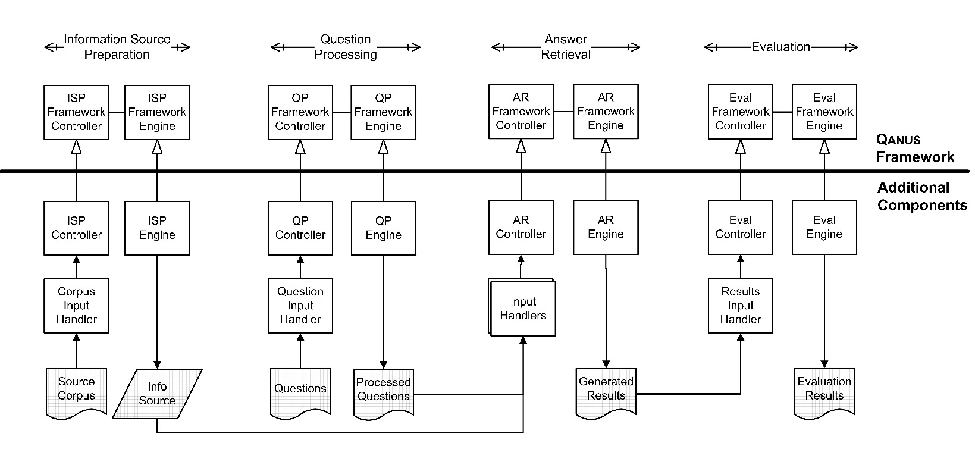
\includegraphics{graficos/Quanus}
  \caption{El framework Quanus y la implementación QA-sys}
  \label{fig:Quanus}
\end{figure}


La arquitectura, al igual que la de DeepQA, es la de un pipeline. Este
sistema consta de tres pasos principales, que se ejecutan todos por
separado (off-line): 


\bigskip

\subsection{Preparación de la fuente de información}
Este paso está pensado para preprocesar cualquier base de conocimiento
y dejarla preparada para el paso 3 (retorno de la pregunta). El
framework se propone tan amplio que no hay más especificaciones al
respecto. La implementación puntual asume una base de conocimiento en
formato XML de AQUAINT\footnote{\ } y la incorpora a un índice de
búsquedas Lucene. Este paso incorpora todo el conocimiento que
estará finalmente offline; accesos dinámicos a la web, por ejemplo,
se modelan en el paso 3.


\bigskip

\subsection{Análisis de la pregunta}
Este paso, igualmente genérico, permite la incorporación de
distintos componentes para anotar los tokens de la pregunta con datos
útiles para ser consumidos por el paso 3. Otro procesamiento a
realizar en este paso podría ser la generación de queries
entendibles por los distintos motores de almacenamientos de
información del paso 1. En particular, la implementación trae un
pos-tagger, un ner-tagger y un question classiffier, todos de Stanford.
Hablaremos más de estos componentes más adelante. 


\bigskip

\subsection{Generación de respuestas}
En este paso se utiliza la información generada en la preparación
de la base de información y en el procesamiento de la pregunta para
generar una respuesta. También puede incorporarse accesos a la web y
validaciones de las respuestas candidatas. La implementación concreta
evalúa cada pasaje de los primeros n documentos retornados por Lucene
para la pregunta original con una serie de componentes ad-hoc de
distancia para adjudicar diferentes grados de confiabilidad a los
distintos pasajes. \newline


Además, se provee de un cuarto paso opcional (el sistema de QA está
completo con los tres pasos anteriores), para la fase de desarrollo y
de evaluación de la performance del sistema:\newline


\subsection{Evaluación}

Este paso está pensado para evaluar las respuestas generadas y
presentarlas de un modo conciso en la fase de desarrollo.
Básicamente, cruza las respuestas obtenidas contra unas respuestas
esperadas escritas a mano y presenta el total de respuestas dadas
correctamente.


\bigskip

\subsection{Implementación}

El código está escrito en java y mantiene una interfaz común a
todos los pasos: un controller cuyas responsabilidades son cargar los
componentes y un engine que utiliza los componentes para leer el input,
procesarlo y grabar el resultado. La adaptabilidad del framework está
dada en la posibilidad de incorporar componentes respetando la interfaz
especificada para los mismos o bien, en modificar esta misma interfaz.
Presuntamente, el framework es lo suficientemente abierto para permitir
la implementación de sistemas basados en distintas fuentes de
conocimiento (ontologías, archivos, web) y con distintos modos de
funcionamiento mediante poco esfuerzo de customización.

La implementación llamada QA-sys está desarrollada para correr sobre
el tipo de datos de las evaluaciones TREC 2007 (XML AQUAINT). En el
primer paso, incorpora los XML en este formato a un índice Lucene, en
el segundo paso utiliza anota la pregunta con POS tags, NERs y
clasifica el tipo de respuesta con un clasificador entrenado y luego,
en el tercer paso se busca la pregunta sobre el índice lucene y se
retorna una lista con n documentos rankeados. Estos documentos se
subdividen en pasajes. Luego se aplican diferente algoritmos ad-hoc
dependiendo del tipo de respuesta esperada. \ Por ejemplo, si la
respuesta es un nombre de persona, se ejecuta NER sobre los diferentes
pasajes buscando nombres candidatos, si el tipo esperado es una fecha,
se utilizan expresiones regulares escritas a mano, etc. Finalmente, los
pasajes candidatos se evalúan utilizando heurísticas de proximidad
de los candidatos a la pregunta inicial. Para esto se utilizan
diferentes Scorers que rankean los pasajes según diferentes
características (features) y luego se selecciona alguna priorizando
algunas características sobre otras, dependiendo también del tipo
de respuesta esperada. Por último, el evaluador de resultados mide la
exactitud (\textit{accuracy}): total de respuestas correctas sobre
total de preguntas. QA-sys funciona sólo sobre preguntas del tipo
factoid y, a modo de comparación, el mejor sistema según la TREC
2007, el LymbaPA07 obtuvo un grado de exactitud del 0.706 y el décimo
(Quanta) obtuvo 0.206, mientras que QA-sys logra el 0.119. La
implementación es realmente simple y funciona sólo a modo de
ilustración de lo que puede construirse sobre el framework. 

\bigskip

\section{Otros sistemas de QA: OpenEphyra, Aranea y Just.Ask}

\bigskip

El paper describe las arquitecturas de todos los sistemas, si sirve
meter más info

El paper [EPHYRA1] \ busca crear un criterio cuantitativo para comparar
la eficacia de distintos pasos de Just.Ask, Open Ephyra y Aranea
basándose en la arquitectura \textit{pipeline de tres pasos}
compartida por todos. Los tres sistemas, por lo demás, están
basados en la web, utilizando distintas APIs de buscadores o bien
analizando los resultados de la interfaz de usuario de los mismos. 

El primer ítem importante a destacar de este trabajo, es que, al
momento de la experimentación \textbf{Aranea no funcionaba más y
estaba discontinuado}\footnote{\ (Resaltado en Sección 8, muy
concluyente).\par }\textbf{. }El autor se comunicó con el responsable
del proyecto que corroboró que las APIs de los buscadores en los que
se basaba Aranea cambiaron y no había interés en readaptar el
código para que vuelva a funcionar. Las comparaciones que logró
entre Just.Ask y Open Ephyra son interesantes y concluyentes a favor de
la performance de OpenEphyra. 

(Freeling \ + Cambio de Base + Rigidez)

\section{Algunos ejemplos académicos}

\begin{itemize}
\item Watson: \cite{WATSON1} y \cite{WATSON2}
\item Qanus: \cite{QANUS1}

\item Ephyra: \cite{EPHYRA1}
\item Varios de QA: Yago \cite{YAGO-QA1}, sobre una teoria de QA como interfaz a DBs: \cite{QADB1}. Corpus: \cite{TRAIN-QA1}, qall-me: \cite{QALL-ME1}, practical QA: \cite{QAS1}, simple QA: \cite{QAS2} y Surface de Ravishandran: \cite{SURF1}. Introducción a QA: \cite{QA1} y \cite{QA2} y \cite{QA3}
\item Aranea: \cite{ARANEA1} (no leido)
\item Passage retrieval evaluation: \cite{PASSAGE1}
\item Evaluacion de las TREC8 (metrica de \cite{QA3} LASSO): \cite{TREC8}
\end{itemize}

\section{Conclusiones}
